% !TEX root = ./report.tex

\clearpage
\section{Background}
\label{background}

\subsection{The Regionalized Value-State Dependence Graph}
\label{background:RVSDG}

The \textit{Regionalized Value-State Dependence Graph} (RVSDG) is a
\textit{directed acyclic graph} (DAG) \textit{demand-based dependence graph}
(DDG), consisting of nodes representing computations and edges representing the
dependencies between nodes. Each node has inputs and outputs connected through
edges. The arity and order of inputs and outputs depend on the operation the
node represents.

The RVSDG has two kinds of nodes, and two kinds of edges: simple- and complex-
nodes, and data- and state- dependency edges. Simple nodes represent ``basic
operations'', such as addition and subtraction. Complex nodes contain another
RVSDG subgraph, and are also called \textit{regions}.

\subsubsection{Edges}

The RVSDG has two types of edges: data dependence edges, and state dependence
edges, representing data and state dependencies respectively. Data dependence
edges represent a data dependency one node has to another. State dependence
edges are used to preserve the program semantics when it has side-effecting
operations. We use dashed lines in this report to denote state dependence edges
in figures, as shown in Figure~\ref{fig:for_loop_rec_fib_print_ex}.

\subsubsection{Nodes}

The RVSDG has two kinds of nodes: simple nodes are used in an RVSDG to represent
simple operations, such as addition and subtraction.

The report puts emphasis on the simple node \applyNode .

A special case of the simple nodes listed in this report is the
\textit{apply}-node, which always has an edge linking a $\phi$-region or
$\lambda$-node as first input. The arity and order of the rest of the
\textit{apply}-node's inputs must match the order and arity of the inputs for
the $\lambda$-node linked directly or through a $\phi$-region. While a
$\phi$-region or $\lambda$-node may each link to several \textit{apply}-nodes
representing the same function call, an \textit{apply}-node can (and must)
always have a link to one $\phi$-region or $\lambda$-node as its first input.

The complex nodes of an RVSDG relevant for this are as follows:

\begin{itemize}

\item \textbf{$\gamma$-nodes: N-way statements}

\textit{$\gamma$-nodes} represent conditional statements. Each $\gamma$-node has
a predicate as input. All other edges passing into the $\gamma$-node are edges
its subsection's subgraph(s) depend upon. All subsections must have the same
order and arity of inputs and outputs, even if the subgraph in each case does
not depend on all of the inputs, or modify all of the outputs.

A $\gamma$-node most closely represents a \textit{switch-case} without fall-
through in each case. Each case of the switch statement corresponds then with a
subsection of the $\gamma$-node.

Hence, a simple \textit{if-statement} with no else-clause can be represented by
a $\gamma$-node with two subsections. The true subsection containing the RVSDG
subgraph representing the body of the if-statement. The false subsection of the
$\gamma$-node simply routing through all inputs straight out again unmodified.

How nested $\gamma$-nodes can represent the semantics of \textit{if, else if,
else} is shown in Figure~\ref{fig:nested_ifs}.

\begin{centering}
	\noindent\begin{minipage}{0.36\textwidth}
		\begin{lstlisting}[label={lst:nested_ifs}, style=customcpp]
if(smth){
	//do something 1
} else if(smth2){
	//do something 2
} else{
	//do something else
}
		\end{lstlisting}
	\end{minipage}
	\noindent\begin{minipage}{0.55\textwidth}
		\captionsetup{type=figure}
		\includegraphics[width=\textwidth]{figures/if_elseif_else_example}
	\end{minipage}
	\captionof{figure}{Minimal example of two nested $\gamma$-nodes representing
the the same semantics as the C/C++ pseudo code on the left.}
	\label{fig:nested_ifs}
\end{centering}

\item \textbf{$\theta$-nodes: Tail-controlled loops}

\textit{$\theta$-nodes} represent tail controlled loops. Like with the
$\gamma$-node, its input is the predicate. All other edges are the dependencies
needed by its subgraph(s) representing the statements in the body of the loop.

In C/C++ $\theta$-nodes are equivalent to \textit{do-while loops} containing the
subgraph representing of the body of the loop inside the node. Other loops, such
as \textit{for-loops}, can be represented by putting a $\theta$-node inside of
the \textit{true} clause of a $\gamma$-node with no subgraph in the subsection
of the \textit{false} clause. The $\gamma$- and $\theta$-nodes both need to have
the exact same predicate, and same dependencies on the predicate, if the
combined subgraph is to represent a for-loop.

See Figure~\ref{fig:for_loop_rec_fib_print_ex} for an example of a $\theta$-node
with corresponding C/C++ code in Listing~\ref{lst:for_loop_rec_fib_print_ex}.
The stippled directed edges in Figure~\ref{fig:for_loop_rec_fib_print_ex} denote
state dependencies between nodes.

\begin{lstlisting}[label={lst:for_loop_rec_fib_print_ex}, style=customcpp,
caption={C/C++ code corresponding to the RVSDG subgraph in
Figure~\ref{fig:for_loop_rec_fib_print_ex}.}]
int recursive_fibonacci(int n){
	if (n == 1 || n == 0){
		return n;
	}
	return recursive_fibonacci(n-1) + recursive_fibonacci(n-2);
}

for(int i = 0; i < 7; i++){
	std::cout << "Fib #" << i << ": " << recursive_fibonacci(i) << std::endl;
}
\end{lstlisting}
\vspace{-4\parskip} %http://tex.stackexchange.com/q/40863
\newpage

\begin{figure}[ht!]
	\centering
	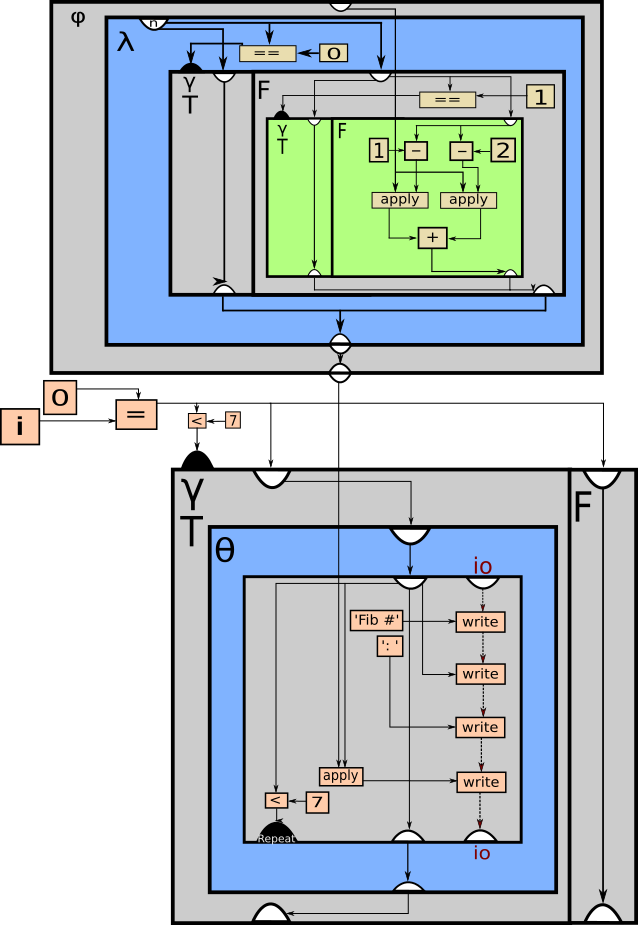
\includegraphics[width=\textwidth]{figures/for-loop-printf-rec_fib-example}
	\caption{A program consisting of a $\theta$-node looping 7 iterations,
calculating and printing the 7 first Fibonacci numbers. The \applyNode ~contained
in the $\theta$-node links to the same recursive Fibonacci function as in
Figure~\ref{fig:rec_fib_phi}.}
	\label{fig:for_loop_rec_fib_print_ex}
\end{figure}

\clearpage
\item \textbf{$\lambda$-nodes: Functions}

\textit{$\lambda$-nodes} represent functions, and these are paired with at least
one \textit{apply}-node. There is only one $\lambda$-node per function in the
program the RVSDG represents. As with the other complex nodes, the order and
arity of inputs needed for the subgraph of the $\lambda$-node need to match the
order and arity of the inputs and edges in its corresponding
\textit{apply}-nodes. However, there are never any RVSDG nodes connected to the
inputs of a $\lambda$-node. They serve rather as placeholders, telling the
\textit{apply}-nodes the arity and order of the inputs of the $\lambda$-node
linked to each \textit{apply}-node.

As previously mentioned, \textit{apply}-nodes represent the call sites of the
function represented by the $\lambda$-node. All \textit{apply}-nodes have an
edge linking it to its corresponding $\lambda$-node as its first input. Hence,
the only dependence edges going \textit{from} a $\lambda$-node are the edges
linking it to its \textit{apply}-nodes.

However, if the $\lambda$-node represents a recursive function, it will reside
inside of a $\phi$-region. It's still linked with all \textit{apply}-nodes
representing calls to the function, but instead of being directly linked, like
$\lambda$-nodes representing non-recursive functions, the \textit{apply}-nodes
are linked to an output of the $\phi$-region corresponding to the correct
$\lambda$-node contained in the $\phi$-region. Figure~\ref{fig:rec_fib_phi}
illustrates how a recursive $\lambda$-node is contained by a $\phi$-region in a
RVSDG.

\item \textbf{$\phi$-regions: Recursive environments}

\textit{$\phi$-regions} contain $\lambda$-nodes representing recursive
functions. $\phi$-regions, like $\lambda$-nodes, have no inputs for themselves.
They may have inputs representing dependencies of their internal RVSDG
subgraphs. The functions represented by $\lambda$-nodes contained in a
$\phi$-node behave recursively either through calling themselves, or two or more
calling each other (mutually recursive).

Internally, and externally, they have two sets of ``outputs''. The external ones
can be considered ``actual'' outputs, enable links to any external
\textit{apply}-nodes representing calls to $\lambda$-nodes residing inside of
the $\phi$-region. The internal ``outputs'' are used to link the internal
\textit{apply}-nodes, which give the $\lambda$-nodes contained by the
$\phi$-region their recursive behaviour without breaking the DAG properties of
the RVSDG.

Hence, the $\lambda$-nodes inside of a $\phi$-region are not directly linked to
any \textit{apply}-nodes, like $\lambda$-nodes representing non-recursive
functions. Instead, the link used by non-recursive $\lambda$-nodes goes to the
$\phi$-region itself, enabling the aforementioned linking between a
$\phi$-region and internal/external \textit{apply}-nodes.
Figure~\ref{fig:rec_fib_phi} illustrates how a $\phi$-node containing the
representation of a recursive fibonacci function would look like in an RVSDG,
and Figure~\ref{fig:for_loop_rec_fib_print_ex} illustrates how
\textit{apply}-nodes can be linked with a $\phi$-region.

\end{itemize}

\begin{lstlisting}[label={lst:rec_fib_phi}, style=customcpp,
caption={C/C++ code corresponding to the RVSDG subgraph in
Figure~\ref{fig:for_loop_rec_fib_print_ex}, which represents a simple recursive
fibonacci function.}]
int recursive_fibonacci(int n){
	if (n == 1 || n == 0){
		return n;
	}
	return recursive_fibonacci(n-1) + recursive_fibonacci(n-2);
}
\end{lstlisting}
\vspace{-4\parskip} %http://tex.stackexchange.com/q/40863

\begin{figure}[h!]
	\centering
	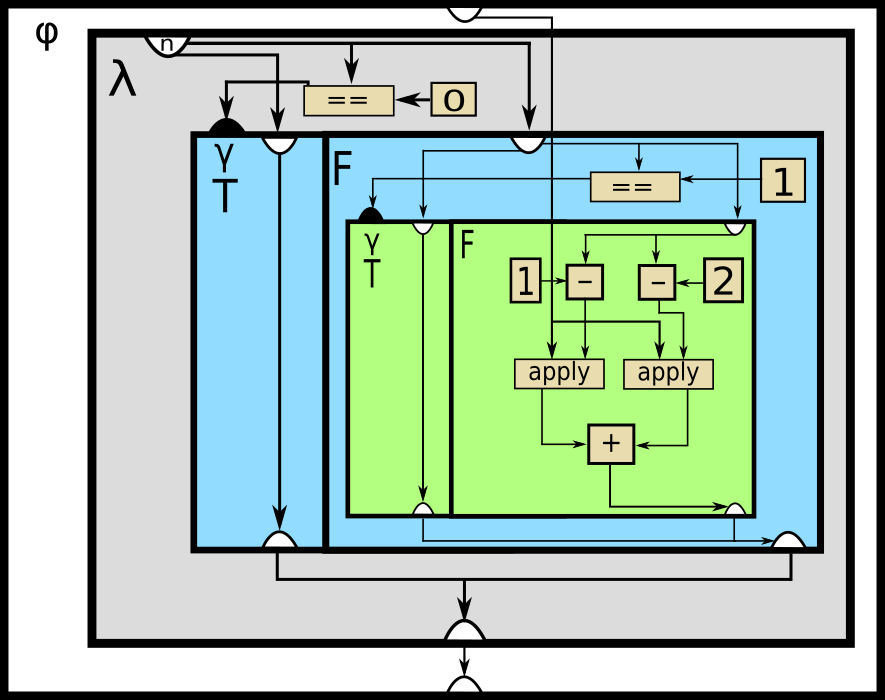
\includegraphics[width=\textwidth]{figures/recursive_fibonacci}
	\caption{A $\phi$-node containing a $\lambda$-node representing a recursive
version of a function producing the $n$ first numbers in the Fibonacci series.}
	\label{fig:rec_fib_phi}
\end{figure}
